\documentclass[border=5pt]{standalone}
\usepackage{pgfplots}
\pgfplotsset{compat=1.18}
\usepackage{siunitx}
\usepackage{tikz}
\usetikzlibrary{calc}

\definecolor{trainColor}{RGB}{31,119,180}
\definecolor{valColor}{RGB}{255,127,14}

\begin{document}
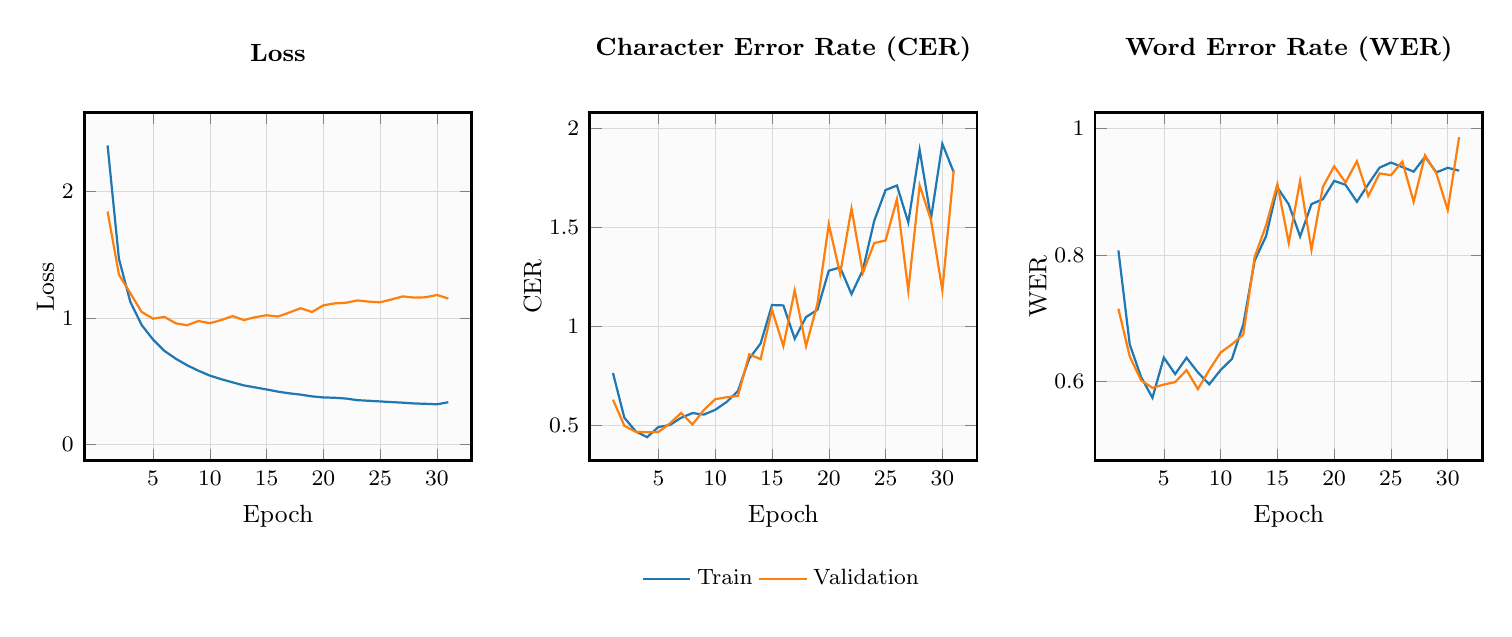
\begin{tikzpicture}[remember picture]

    % Graph 1: Loss
    \begin{axis}[
        name=plot1,
        width=6.5cm,
        height=6cm,
        xlabel={Epoch},
        ylabel={Loss},
        ylabel style={yshift=-0.15cm},
        xmin=0.5, xmax=31.5,
        ymin=0, ymax=2.5,
        xtick={5,10,15,20,25,30},
        grid=both,
        grid style={line width=.1pt, draw=gray!10},
        major grid style={line width=.2pt,draw=gray!30},
        title={Loss},
        axis background/.style={fill=gray!3},
        title style={yshift=3mm, font=\small\bfseries},
        label style={font=\small},
        tick label style={font=\footnotesize},
        line width=1pt,
        enlarge x limits=0.05,
        enlarge y limits=0.05,
        every axis plot/.append style={no markers}, % Removed point markers
        legend to name=commonlegend,
        legend columns=2,
        legend style={draw=none, fill=none, font=\footnotesize}
    ]
        % Train
        \addplot[color=trainColor, thick] coordinates {
            (1, 2.3660) (2, 1.4690) (3, 1.1299) (4, 0.9464) (5, 0.8319)
            (6, 0.7422) (7, 0.6801) (8, 0.6283) (9, 0.5850) (10, 0.5467)
            (11, 0.5181) (12, 0.4932) (13, 0.4689) (14, 0.4529) (15, 0.4370)
            (16, 0.4196) (17, 0.4063) (18, 0.3961) (19, 0.3823) (20, 0.3739)
            (21, 0.3712) (22, 0.3650) (23, 0.3523) (24, 0.3474) (25, 0.3422)
            (26, 0.3371) (27, 0.3323) (28, 0.3262) (29, 0.3236) (30, 0.3194)
            (31, 0.3359)
        };
        
        % Validation
        \addplot[color=valColor, thick] coordinates {
            (1, 1.8435) (2, 1.3443) (3, 1.1983) (4, 1.0496) (5, 0.9964)
            (6, 1.0106) (7, 0.9597) (8, 0.9445) (9, 0.9781) (10, 0.9606)
            (11, 0.9848) (12, 1.0169) (13, 0.9854) (14, 1.0082) (15, 1.0235)
            (16, 1.0129) (17, 1.0451) (18, 1.0789) (19, 1.0492) (20, 1.1019)
            (21, 1.1173) (22, 1.1223) (23, 1.1405) (24, 1.1311) (25, 1.1259)
            (26, 1.1485) (27, 1.1726) (28, 1.1627) (29, 1.1653) (30, 1.1837)
            (31, 1.1560)
        };
        
        \legend{Train, Validation}
    \end{axis}
    
    % Graph 2: CER, positioned to the right of plot1
    \begin{axis}[
        name=plot2,
        at={($(plot1.east)+(1.5cm,0)$)},
        anchor=west,
        width=6.5cm,
        height=6cm,
        xlabel={Epoch},
        ylabel={CER},
        ylabel style={yshift=-0.15cm},
        xmin=0.5, xmax=31.5,
        ymin=0.4, ymax=2.0,
        xtick={5,10,15,20,25,30},
        grid=both,
        grid style={line width=.1pt, draw=gray!10},
        major grid style={line width=.2pt,draw=gray!30},
        title={Character Error Rate (CER)},
        axis background/.style={fill=gray!3},
        title style={yshift=3mm, font=\small\bfseries},
        label style={font=\small},
        tick label style={font=\footnotesize},
        line width=1pt,
        enlarge x limits=0.05,
        enlarge y limits=0.05,
        every axis plot/.append style={no markers} % Removed point markers
    ]
        % Train
        \addplot[color=trainColor, thick] coordinates {
            (1, 0.7628) (2, 0.5367) (3, 0.4676) (4, 0.4383) (5, 0.4897)
            (6, 0.4996) (7, 0.5364) (8, 0.5602) (9, 0.5525) (10, 0.5765)
            (11, 0.6161) (12, 0.6716) (13, 0.8361) (14, 0.9123) (15, 1.1067)
            (16, 1.1048) (17, 0.9362) (18, 1.0461) (19, 1.0828) (20, 1.2804)
            (21, 1.2971) (22, 1.1621) (23, 1.2836) (24, 1.5325) (25, 1.6884)
            (26, 1.7113) (27, 1.5246) (28, 1.8921) (29, 1.5442) (30, 1.9225)
            (31, 1.7787)
        };
        
        % Validation
        \addplot[color=valColor, thick] coordinates {
            (1, 0.6280) (2, 0.4960) (3, 0.4654) (4, 0.4633) (5, 0.4646)
            (6, 0.5074) (7, 0.5608) (8, 0.5024) (9, 0.5759) (10, 0.6303)
            (11, 0.6402) (12, 0.6466) (13, 0.8574) (14, 0.8329) (15, 1.0825)
            (16, 0.8991) (17, 1.1813) (18, 0.8993) (19, 1.1128) (20, 1.5151)
            (21, 1.2645) (22, 1.5951) (23, 1.2696) (24, 1.4202) (25, 1.4333)
            (26, 1.6420) (27, 1.1797) (28, 1.7128) (29, 1.5364) (30, 1.1814)
            (31, 1.7880)
        };
    \end{axis}
    
    % Graph 3: WER, positioned to the right of plot2
    \begin{axis}[
        name=plot3,
        at={($(plot2.east)+(1.5cm,0)$)},
        anchor=west,
        width=6.5cm,
        height=6cm,
        xlabel={Epoch},
        ylabel={WER},
        ylabel style={yshift=-0.15cm},
        xmin=0.5, xmax=31.5,
        ymin=0.5, ymax=1.0,
        xtick={5,10,15,20,25,30},
        grid=both,
        grid style={line width=.1pt, draw=gray!10},
        major grid style={line width=.2pt,draw=gray!30},
        title={Word Error Rate (WER)},
        axis background/.style={fill=gray!3},
        title style={yshift=3mm, font=\small\bfseries},
        label style={font=\small},
        tick label style={font=\footnotesize},
        line width=1pt,
        enlarge x limits=0.05,
        enlarge y limits=0.05,
        every axis plot/.append style={no markers} % Removed point markers
    ]
        % Train
        \addplot[color=trainColor, thick] coordinates {
            (1, 0.8072) (2, 0.6585) (3, 0.6070) (4, 0.5742) (5, 0.6378)
            (6, 0.6117) (7, 0.6375) (8, 0.6144) (9, 0.5955) (10, 0.6181)
            (11, 0.6357) (12, 0.6903) (13, 0.7912) (14, 0.8296) (15, 0.9067)
            (16, 0.8800) (17, 0.8292) (18, 0.8804) (19, 0.8881) (20, 0.9171)
            (21, 0.9109) (22, 0.8840) (23, 0.9117) (24, 0.9381) (25, 0.9461)
            (26, 0.9390) (27, 0.9318) (28, 0.9551) (29, 0.9306) (30, 0.9378)
            (31, 0.9333)
        };
        
        % Validation
        \addplot[color=valColor, thick] coordinates {
            (1, 0.7151) (2, 0.6396) (3, 0.6017) (4, 0.5900) (5, 0.5951)
            (6, 0.5991) (7, 0.6179) (8, 0.5879) (9, 0.6181) (10, 0.6458)
            (11, 0.6588) (12, 0.6744) (13, 0.7970) (14, 0.8466) (15, 0.9119)
            (16, 0.8190) (17, 0.9171) (18, 0.8081) (19, 0.9074) (20, 0.9401)
            (21, 0.9147) (22, 0.9481) (23, 0.8932) (24, 0.9289) (25, 0.9261)
            (26, 0.9476) (27, 0.8841) (28, 0.9574) (29, 0.9288) (30, 0.8711)
            (31, 0.9864)
        };
    \end{axis}

    % Positioning the common legend below all graphs
    \node at ($(plot1.south)!0.5!(plot3.south)+(0,-1.5cm)$) {\pgfplotslegendfromname{commonlegend}};
    
\end{tikzpicture}
\end{document}